\documentclass{article}

\usepackage[utf8]{inputenc}
\usepackage{amsmath}
\usepackage{amssymb}
\usepackage{algorithm}
\usepackage[noend]{algpseudocode}
\usepackage{float}
\usepackage{graphicx}
\usepackage{afterpage}
\begin{document}

\title{Exponential Integrators for PDEs arising in meteorology} 
\maketitle
\author{Harvey Sutton}

\tableofcontents
\newpage

\section {Introduction}
\subsection{Motivation}
%Statement of ODE
In many simulations, it is common to encounter ODEs of the form
\begin{align}
\dot u(t) = Au(t) + R(u) \label{ODE}
\end{align}
Where $A$ is a large sparse matrix and $R$ denotes some nonlinear term.
As a result, finding accurate approximate solutions to these equations is of major importance.\\

%Method of lines
Often ODEs also occur when solving PDEs numerically using the method of lines.
This arrives from discretising the PDE in space yielding an ODE with respect to time, with the form shown in \eqref{ODE}.\\
\subsection{Solvers}
%ODE Solvers
Solving these ODEs numerically works by progressively stepping through time such as with the explicit forward Euler method, which is given as:
\begin{align*}
u(t+\tau) &\approx u(t) + \tau\dot u(t) = u(t) + \tau(Au(t) + R(u(t)))
\end{align*}
for a given step size $h$.
%Exponential Integrators
Another method (and the one we will be focusing on here) employs the use of the exponential integrator, which writes the solution to problem \eqref{ODE} over a given time step as:
\begin{align*}
u(t+\tau) &= e^{Ah}u(t) + \int_0^h e^{A(\tau-z)}N(u(t+z)) dz \label{ODE Solution}\\
&\text{using a simple explicit approach leads to}\\
&\approx e^{Ah}(u(t) + N(u(t))\\
\text{where } e^{A} &= \sum^{\infty}_{i = 0}\frac{A^n}{n!}
\end{align*}
%Computing matrix exponential for A sparse
\subsection{Computing the Matrix Exponential}
An important requirement when using this method is to compute approximations of $e^{A}v$ efficiently and accurately for the given sparse matrix $A$ and vector $v$.
One approach would be first to compute $e^A$ and apply the resulting matrix to the vector $v$.
However, even for sparse $A$, $e^{A}$ will likely be dense. For large $A$ this will result in very high memory usage, which may not be practical when approximating solutions to \eqref{ODE Solution}.
One solution to reduce memory usage is to compute $e^{A}v$ directly without computing $e^{A}$ as an intermediary step.\\
Various methods have been proposed for this such as by Al-Mohy, Awad H. and Higham, Nicholas J\cite{AlMohy2011} and Higham, N. J., and Al-Mohy, A. H. \cite{Higham2010} which is currently used in the Scipy package as \verb|scipy.sparse.linalg.expm_multiply|.
Another class of methods known as Krylov subspace methods have gained traction recently\cite{Moler2003}.
These work by projecting the problem onto a space with fewer dimensions (the Kyrlov subspace), computing the matrix exponential and then transforming back to the original space.
As the matrix exponential will be computed in the lower dimension Kyrlov subspace the computation cost of this step will not be significant.
\subsection{Matrix Free Methods}
Another way of reducing computation time is the use of matrix-free methods.
Frequently to arrive at $\dot u(t) = Au(t) + R(u)$ we will have begun with $\dot u(t) = N(u)$ and linearise around $u(t)$ giving:
\begin{align*}
Au &= DN(u)\\
&\approx \frac{N(u+\epsilon)-N(u)}{\epsilon}
\end{align*}
As a result, we can approximate the action of the matrix  $A$ on $u$ without having to compute $A$ directly or perform a matrix-vector multiplication

\section{Krylov Subspace Methods}
In this section, we will look into existing Krylov subspace methods and then compare how these methods perform for approximating $e^{A}v$.

\subsection{Alogrithms}
The algorithms take a matrix $A\in \mathbb{R}^{n\times n}$, a vector $v \in \mathbb{R}^n$ and an integer $m$ that determines the number of dimensions of the Krylov subspace used.
From these algorithms we will get a matrix $H \in \mathbb{R}^{m\times m}$ and another matrix $V \in \mathbb{R}^{n\times m}$ such that $A \approx VHV^T$ and $VV^T = I$.
From here we get $Av \approx VHV^Tv = VH||v||e_1$.\\
We can apply this to $e^A$ as follows:
\begin{align*}
e^A &= \sum^{\infty}_{i=0}\frac{A^i}{i\!}\\
&= \sum^{\infty}_{i=0}\frac{(VHV^T)^i}{i\!} \\
&= \sum^{\infty}_{i=0}\frac{VH^iV^T}{i\!} \\
&\text {and then when computing $e^Av$ we get}\\
e^Av &= (\sum^{\infty}_{i=0}\frac{VH^iV^T}{i\!})v \\
&= \sum^{\infty}_{i=0}\frac{VH^iV^Tv}{i\!} \\
&= \sum^{\infty}_{i=0}\frac{VH^i||v||e_1}{i\!} \\
&= V(\sum^{\infty}_{i=0}\frac{H^i}{i\!})||v||e_1 \\
&= Ve^H||v||e_1
\end{align*}

Here we give the algorithms for the 2 Krylov subspace methods we will be comparing.
We begin with the Arnoldi algorithm.


\begin{algorithm}[H]
\caption{Arnoldi \cite{Fan2018}} %find better citation
\begin{algorithmic}
\Procedure{Arnoldi}{$A, \hat v_1,m$}
\State $v_0 \gets 0$
\For{$j = 1,2,...,m$}	
\For{$i = 1,2,...,j$}
\State$h_{ij} \gets v_i^T A v_i$
\EndFor
\State$\theta_j \gets Av_j - \sum^j_{i=1} h_{ij}v_i$
\State$h_{j+1,j} \gets ||\theta_j||$
\State$v_{j+1} \gets \theta_j/h_{j+1,j}$
\EndFor
\EndProcedure
\end{algorithmic}
\end{algorithm}
Here V is given by $v_1,...,v_m$ and H is give by $h_1,...,h_m$.\\
The algorithm below is the Lanczos algorithm and it requires a symmetric matrix. \cite{Moler2003}
\begin{algorithm}[H]
\caption{Lanczos \cite{OJALVO1970}}
\begin{algorithmic}
\Procedure{Lanczos}{$A$ symetric$, \hat v_1,m$}
\State $v_0 = 0$
\For{$i = 1,2,...,m$}	
\State$\beta_i \gets || \hat v_i ||$
\State$v_i \gets \hat v_i / || \hat v_i ||$
\State$\alpha_i \gets v_i^T A v_i$
\State$\hat v_{i+1} \gets Av_i - \alpha_iv_i - \beta_iv_{i-1}$
\EndFor
\EndProcedure
\end{algorithmic}
\end{algorithm}
Here $V$ is given by ${v_1,...,v_m}$ and $H$ is tridiagonal with the leading diagonal being $\alpha_1, ..., \alpha_m$ and the upper and lower diagonals being $\beta_2,...,\beta_m$.


\subsection{Numerical Results}
Here we run numerical experiments, computing $e^Av$ for a tridiagonal matrix $A$ of sizes $131072$ and $524288$, where $A$ is a tridiagonal matrix with $2n^2$ along the diagonal and $-n^2$ along the upper and lower diagonals. We will compare the methods with respect to computation time, error and size of the Kyrlov subspace. The error is computed as the Euclidian distance between Scipy and the Krlov subspace method being tested.

\begin{figure}[H]
    \centering
    \begin{minipage}{0.5\textwidth}
       \centering
	  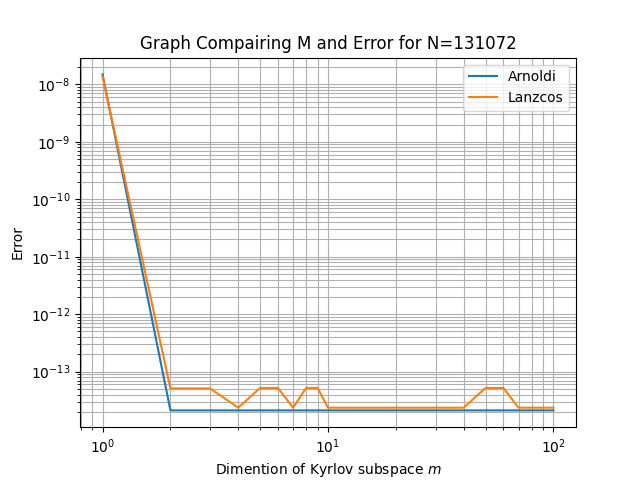
\includegraphics[width=\linewidth]{Plots/M v E Results for N=131072.png}
	  \label{fig:MEe7}
    \end{minipage}\hfill
    \begin{minipage}{0.5\textwidth}
       \centering
	  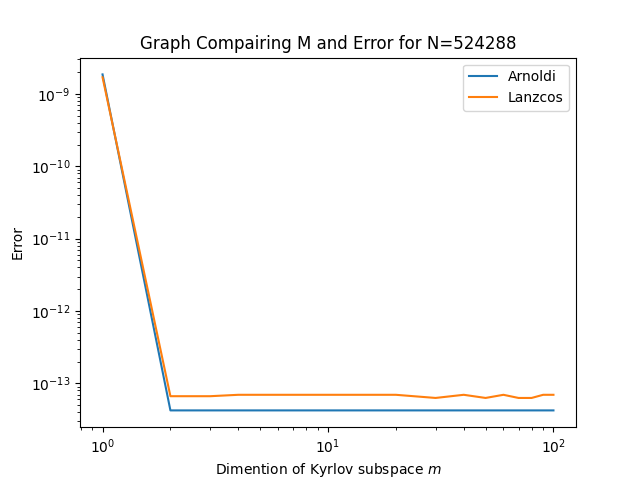
\includegraphics[width=\linewidth]{Plots/M v E Results for N=524288.png}
	  \label{fig:MEe6}
    \end{minipage}
\end{figure}
\begin{figure}[H]
    \centering
    \begin{minipage}{0.5\textwidth}
       \centering
	  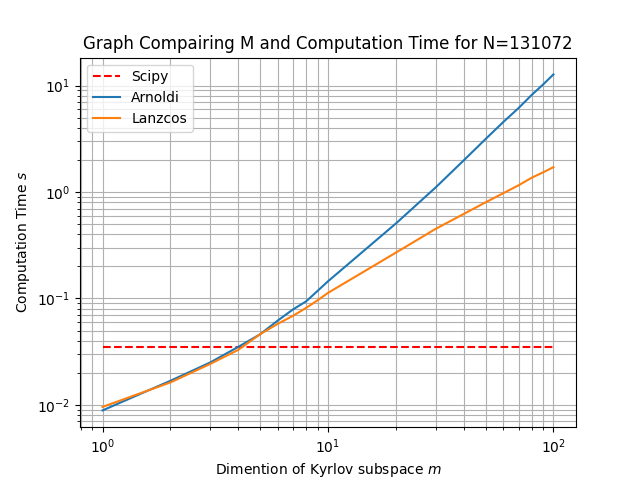
\includegraphics[width=\linewidth]{Plots/M v Comp Time Results for N=131072.png}
	  \label{fig:MEe7}
    \end{minipage}\hfill
    \begin{minipage}{0.5\textwidth}
       \centering
	  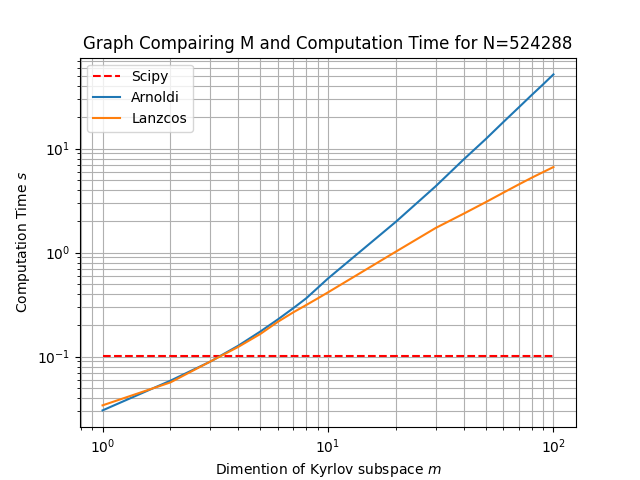
\includegraphics[width=\linewidth]{Plots/M v Comp Time Results for N=524288.png}
	  \label{fig:MEe6}
    \end{minipage}
\end{figure}
\begin{figure}[H]
    \centering
    \begin{minipage}{0.5\textwidth}
       \centering
	  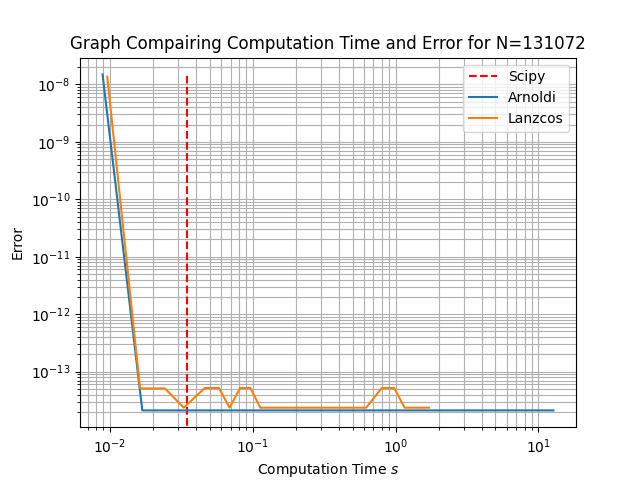
\includegraphics[width=\linewidth]{Plots/Comp Time v E Results for N=131072.png}
	  \label{fig:MEe7}
    \end{minipage}\hfill
    \begin{minipage}{0.5\textwidth}
       \centering
	  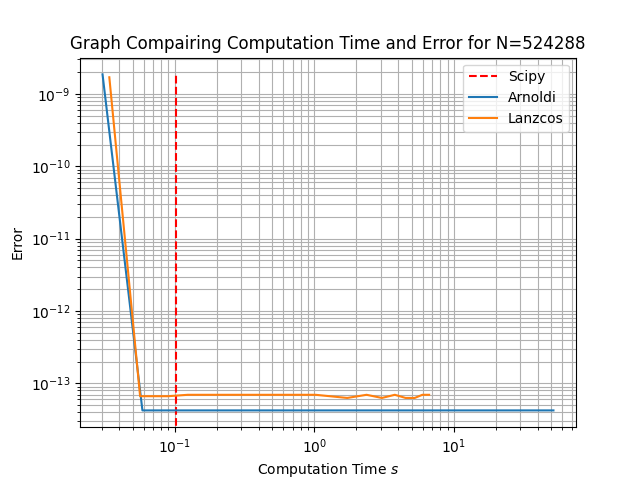
\includegraphics[width=\linewidth]{Plots/Comp Time v E Results for N=524288.png}
	  \label{fig:MEe6}
    \end{minipage}
\end{figure}
These results show that the Lanzcos algorithm outperforms the Arnoldi algorithm in both convergence rate and computational time.

Below we compare the time required for the different algorithms to get below an error of $10^6$ and $10^{10}$ when computing $e^Av$ for various matrix sizes.
\begin{figure}[H]
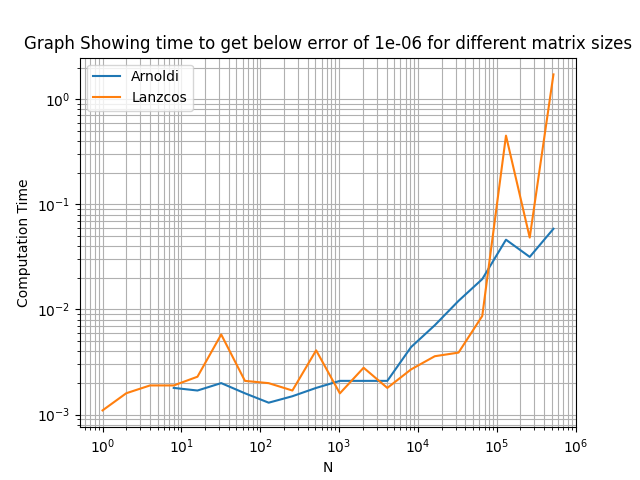
\includegraphics[width=\linewidth]{Plots/time to get below an error of 1e-06.png}
\end{figure}
\begin{figure}[H]
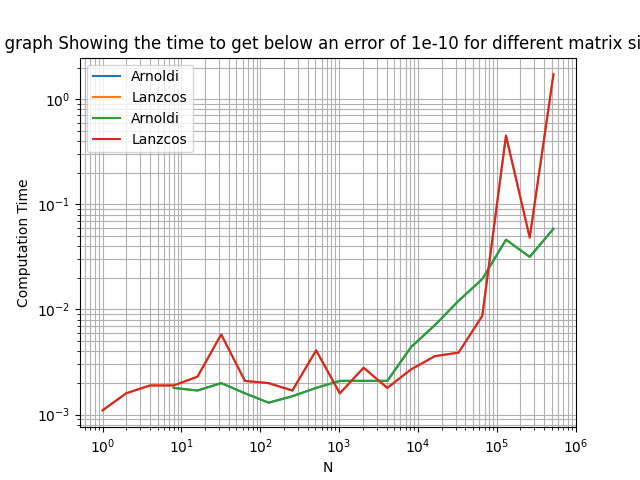
\includegraphics[width=\linewidth]{Plots/time to get below an error of 1e-10.png}
\end{figure}
Again we continue to see that the Lanzcos algorithm outperforms the Arnodli algorithm.

\section{Application to Finite Element Methods}
Here we discuss the application of the exponential integrator to finite element methods.

We begin with a finite element problem in the weak form with $V_h$ a finite-dimensional space.
\begin{align*}
\int \frac d{dt}u(t,x) v_j - R(u) v_j dx &= \mathcal{L}(u,v)\text{Where $v_j$ is a basis of $V_h$}\\
\text{substituting in } u(t,x) &= \sum_{i=1}^n u_i(t)v_i(x)\\
\text{we get } \int\sum_{i=1}^n(\frac d{dt}u_i(t)v_i(x)v_j(x))dx - R(u)v_j(x)dx &= \sum_{i=1}^n u_i(t)\mathcal{L}(v_i(x)v_j(x))\\
\frac d{dt}u_i(t)\sum_{i=1}^n\int v_i(x)v_j(x)dx - \int R(u)v_j(x)dx &= \sum_{i=1}^n u_i(t)\mathcal{L}(v_i(x)v_j(x))\\
\text{setting } S_{ij} &= \mathcal{L}(v_i(x)v_j(x))\\
R_j &= \int R(u)v_j(x)dx\\
M &= \int v_i(x)v_j(x)dx\\
\text{We get}\\
M\frac d{dt}u(t) - R &= Lu\\
\frac d{dt}u(t) &= M^{-1}(Lu + R(u))
\end{align*}
A clear limiting factor when computing $M^{-1}(Lu + R(u))$ is taking the inverse of $M$, the matrix.
One way around this is to perform mass lumping on the matrix, where we sum up the values along each row and place them along the diagonal.
From here computing the inverse is trivial.

\subsection{Numerical Results}
We will now look at the application of the exponential integrator to numerical problems.

We ran our tests over several $N\times N$ grids for various values of $N$ and a selection of values for our time step $\tau$.
There is an initial "seeding" phase where we use a predetermined stepper to compute an approximation from time $t=0$ to a predetermined seed time $t_s$ and with a seeding time step $\tau_s$ producing an approximation at the seed time of $u_s$.
From here we can test our different steppers beginning at time $t_s$ with initial condition $u_s$ using a time step $\tau$ and run until an end time $t_e$.

\subsubsection{Parabolic Problem}
Here we look at the results for a Parabolic Problem given in the weak form below:
\begin{align*}
\text{with exact solution }\hat u(t,x) &= cos(4\pi t)cos(2\pi x_0) \text{ we have}\\
\int \partial_tu v dx&= a(u,v) - l(v)\\
\text{where }a(u,v) &= \int \nabla u \cdot \nabla v + u \cdot v dx\\
\text{and }l(v) &= \int\partial_tu - \nabla \cdot \nabla \hat u)  v_0\\
&+\hat u \cdot vdx\\
&+\int \nabla \hat u \cdot n v_0 dx
\end{align*}

We set $t_s = 0$ and $t_e = 0.02$ and test with $\tau = 2\times 10^{-4}, 1\times 10^{-4}, 5\times 10^{-5}, 2.5\times 10^{-5}, 1.25\times 10^{-5}$.
For grid sizes, we use $N\times N$ with $N = 10,30,60$.

The metrics we will be comparing are the L2 error given by $\int |u_e - \hat u|$ and the number of calls to the operator $N$ (as we are using a matrix-free method).
We present the results for the Arnoldi, Lanczos, Kipops\cite{Gaudreault2018} and Backward Euler methods.

\begin{figure}[H]
	  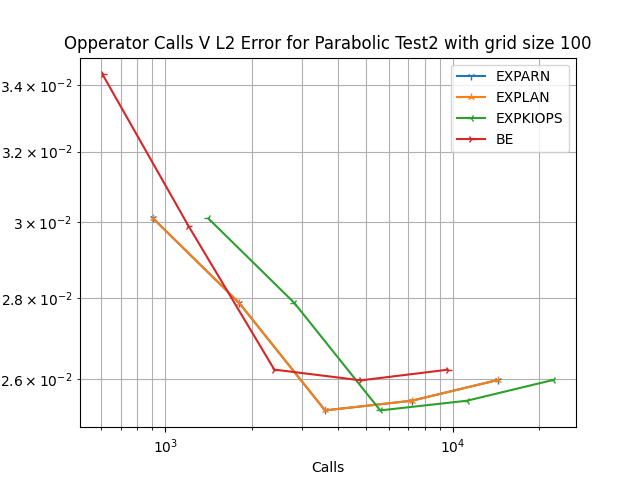
\includegraphics[width=\linewidth]{FEMethodPlots/Operator Calls V Error for Parabolic Test2 with grid size 100.png}
\end{figure}
\begin{figure}[H]
	  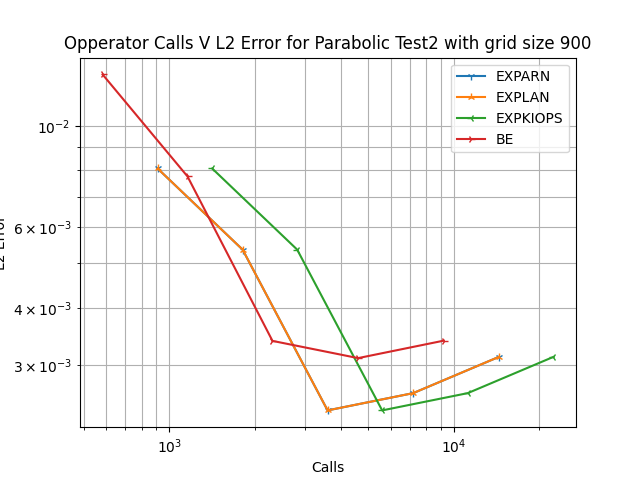
\includegraphics[width=\linewidth]{FEMethodPlots/Operator Calls V Error for Parabolic Test2 with grid size 900.png}
\end{figure}
\begin{figure}[H]
	  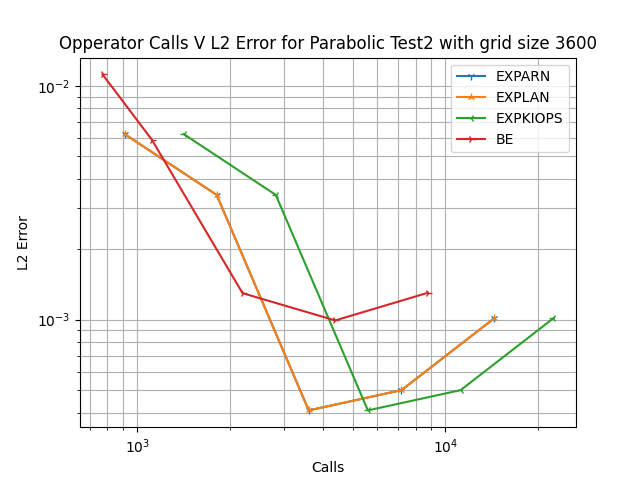
\includegraphics[width=\linewidth]{FEMethodPlots/Operator Calls V Error for Parabolic Test2 with grid size 3600.png}
\end{figure}

From this, we see that for about $1.25\times 10^{3}$ calls to the operator, we achieve a lower error than the backward-euler method was able to.
This corresponds to a tau of $ 5\times 10^{-5}$.
We also observe that after this value, error for all methods plateaus and even increases.

\subsubsection{Allen Cahn}
Here we apply the same exponential integrator methods as above to the Allan Cahn equations.
We give the Allen Cahn equations in weak form below

\begin{align*}
\int \partial_tu v dx &= a(u,v)\\
\text {where } a(u,v) &= \int 10^{-4} \nabla u \cdot \nabla v + (u^2-1)uv dx
\end{align*}

For computing our seed we have $t_s = 4$ and use $\tau = 10^{-2}$ with the Backward Euler method.
For the true value $\hat u$ we use the Backward Euler method to approximate it with $\tau = 10^{-4}$.
We set $t_s = 4$ and $t_e = 50$ and test with $\tau = 2.5\times 10^{-2}$.
For grid sizes, we use $N\times N$ with $N = 60$.


We provide the plot of the seed and at times $t = 20, 50$ for the different methods. 

\begin{figure}[H]
	\centering
	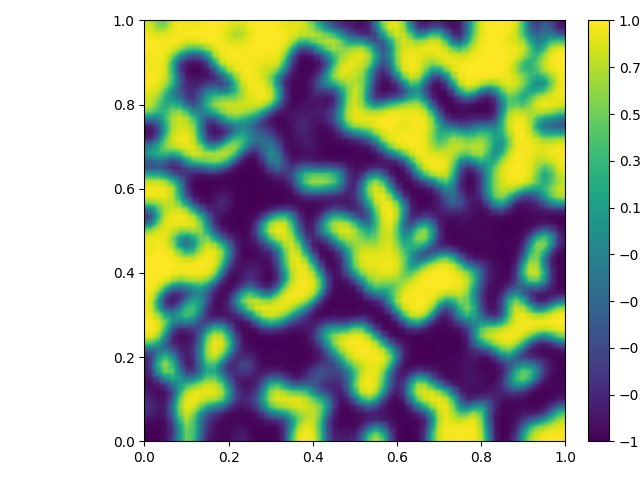
\includegraphics[width=\linewidth]{FEPics/Allen Cahn Test2_60x60_0.025_Seed BE_EndTime=50.png}
	\caption{Seed $t=4$}
\end{figure}
\begin{figure}[H]
    \centering
    \begin{minipage}{0.5\textwidth}
       \centering
	  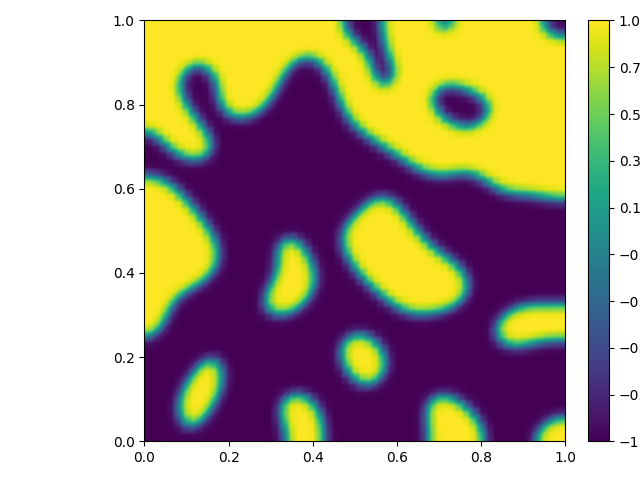
\includegraphics[width=\linewidth]{FEPics/Allen Cahn Test2_60x60_0.025_Target BE_EndTime=20.png}
	  \caption{True $t=20$}
    \end{minipage}\hfill
    \begin{minipage}{0.5\textwidth}
       \centering
	  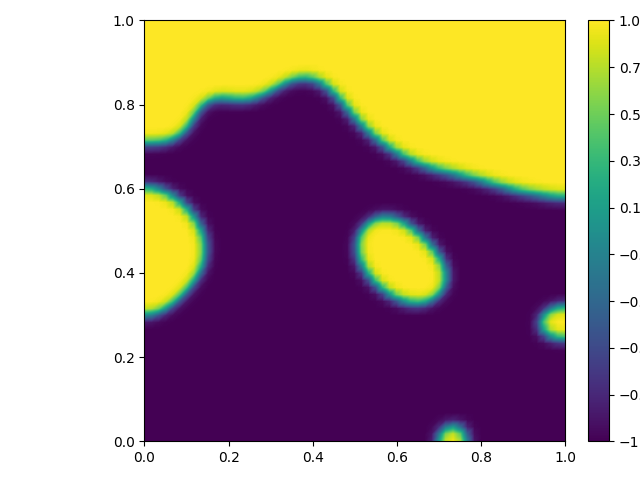
\includegraphics[width=\linewidth]{FEPics/Allen Cahn Test2_60x60_0.025_Target BE_EndTime=50.png}
	  \caption{True $t=50$}
    \end{minipage}
\end{figure}
\begin{figure}[H]
    \centering
    \begin{minipage}{0.5\textwidth}
       \centering
	  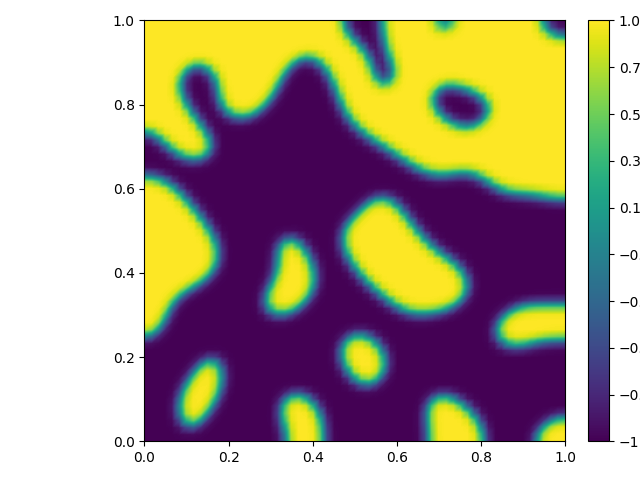
\includegraphics[width=\linewidth]{FEPics/Allen Cahn Test2_60x60_0.025_BE_EndTime=20.png}
	  \caption{Backward Euler $t=20$}
    \end{minipage}\hfill
    \begin{minipage}{0.5\textwidth}
       \centering
	  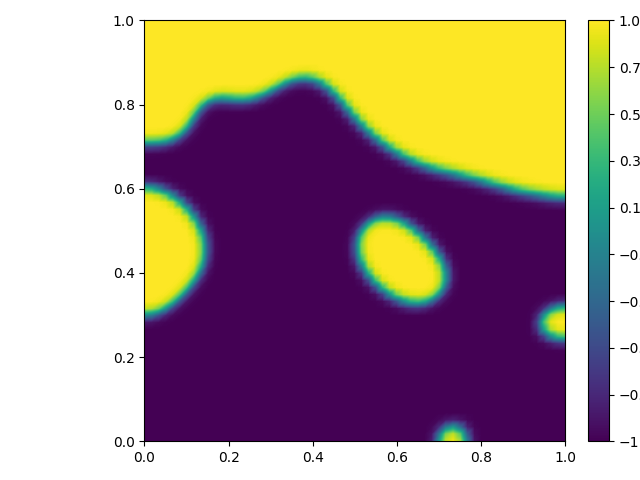
\includegraphics[width=\linewidth]{FEPics/Allen Cahn Test2_60x60_0.025_BE_EndTime=50.png}
	  \caption{Backward Euler$t=50$}
    \end{minipage}
\end{figure}
\begin{figure}[H]
    \centering
    \begin{minipage}{0.5\textwidth}
       \centering
	  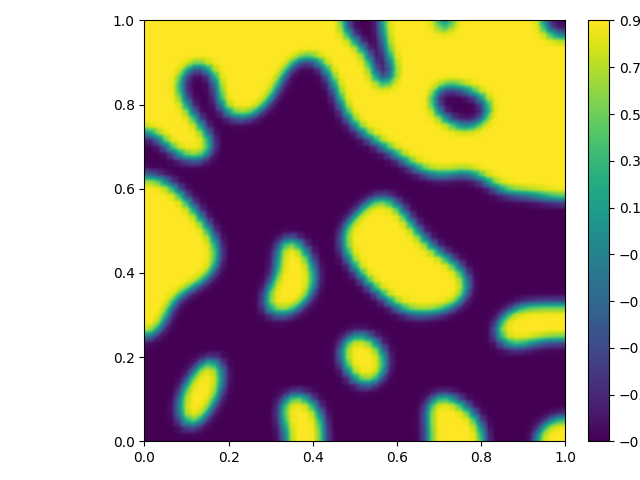
\includegraphics[width=\linewidth]{FEPics/Allen Cahn Test2_60x60_0.025_EXPARN_EndTime=20.png}
	  \caption{Arnoldi $t=20$}
    \end{minipage}\hfill
    \begin{minipage}{0.5\textwidth}
       \centering
	  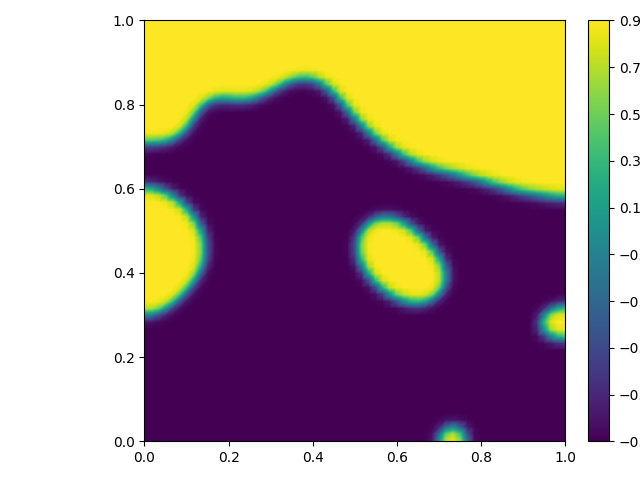
\includegraphics[width=\linewidth]{FEPics/Allen Cahn Test2_60x60_0.025_EXPARN_EndTime=50.png}
	  \caption{Arnoldi $t=50$}
    \end{minipage}
\end{figure}
\begin{figure}[H]
    \centering
    \begin{minipage}{0.5\textwidth}
       \centering
	  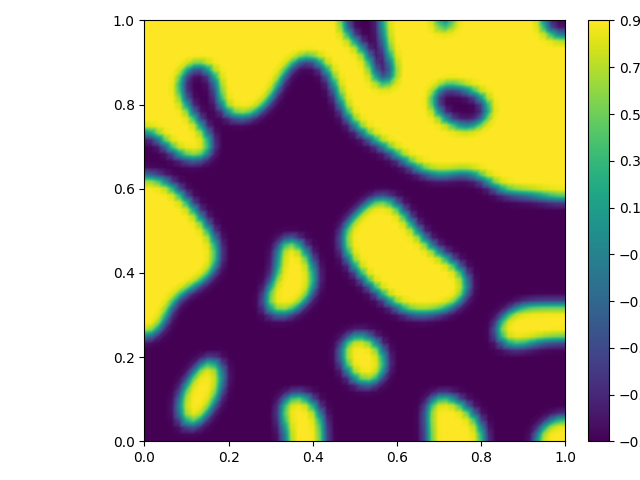
\includegraphics[width=\linewidth]{FEPics/Allen Cahn Test2_60x60_0.025_EXPLAN_EndTime=20.png}
	  \caption{Lanzcos $t=20$}
    \end{minipage}\hfill
    \begin{minipage}{0.5\textwidth}
       \centering
	  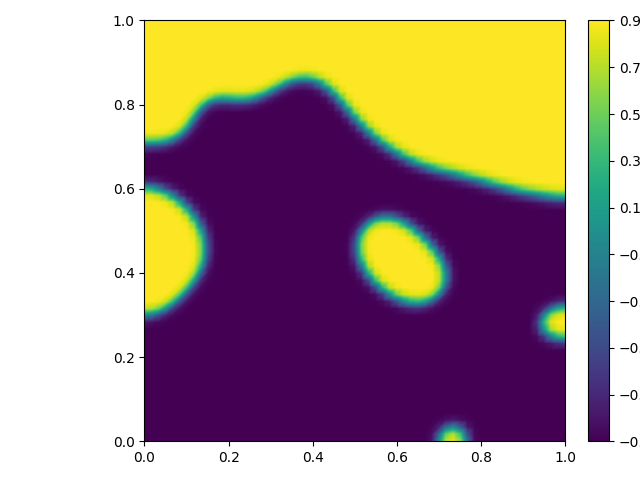
\includegraphics[width=\linewidth]{FEPics/Allen Cahn Test2_60x60_0.025_EXPLAN_EndTime=50.png}
	  \caption{Lanzcos $t=50$}
    \end{minipage}
\end{figure}
\begin{figure}[H]
    \centering
    \begin{minipage}{0.5\textwidth}
       \centering
	  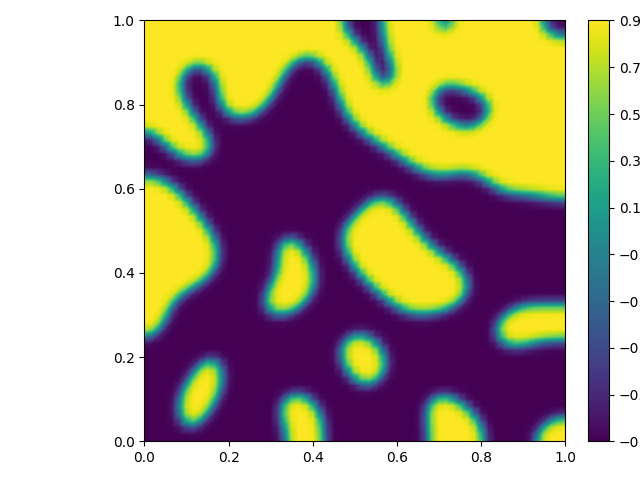
\includegraphics[width=\linewidth]{FEPics/Allen Cahn Test2_60x60_0.025_EXPKIOPS_EndTime=20.png}
	  \caption{Kiops $t=20$}
    \end{minipage}\hfill
    \begin{minipage}{0.5\textwidth}
       \centering
	  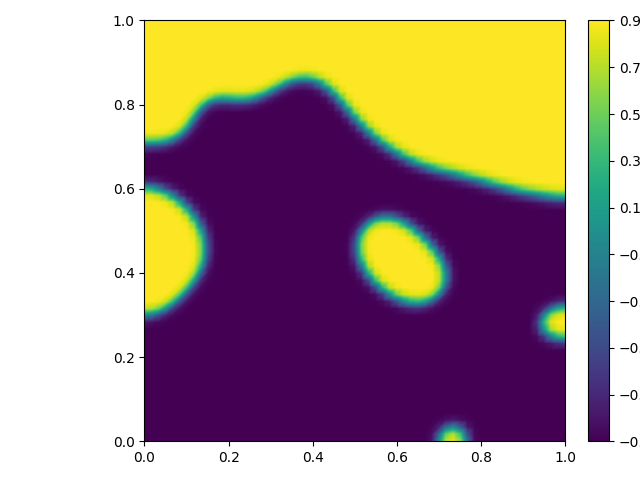
\includegraphics[width=\linewidth]{FEPics/Allen Cahn Test2_60x60_0.025_EXPKIOPS_EndTime=50.png}
	  \caption{Kiops $t=50$}
    \end{minipage}
\end{figure}

The plots for different methods appear to be largely similar to each other.

\section{Conclusion}
Kyrlov subspace methods for computing the action of the matrix exponential on the vector appear to outperform some already commonly used methods such as those used in the scipy library regarding computation time. As a result, when applied to the numerical solutions of PDEs via finite element methods with the use of exponential integrators, we see that Krylov subspace methods appear to be able to achieve a lower minimum L2 error when applied to parabolic problems than the Backward Euler method, especially for finer grid spacing, implying that they may be more suitable for finner grid spacings.
We also see that when applied to the Allen Cahn equations we achieve approximately similar results to the Backward Euler method suggesting that they are also useful for this application.

\section{Outlook}
Further areas requiring investigation include:
Finding how many dimensions are necessary for the Kyrlov subspace to achieve a good approximation for a given problem. Kiops attempts to calculate an optimal size but the Arnoldi and Lanzcos methods achieved comparable results for a lower dimension and were therefore faster.


\clearpage
\newpage
\bibliographystyle{plain}
\bibliography{References.bib}

\end{document}